\documentclass{beamer}
\usetheme[bgphoto]{polimi} 

\usepackage[utf8]{inputenc}
\usepackage{algorithm}
\usepackage{ifxetex}
\usepackage{amsmath}
\usepackage{graphicx} 

\ifxetex
\usepackage{fontspec}
\setsansfont{Arial}[Scale=0.8]
\fi


\title{High Performance Scientific Computing for \\ Aerospace Project}
\subtitle{Progress Update: Solvers \& Parallelization}
\date{December 14th, 2025}


\begin{document}
	

	\begin{frame}
		\maketitle
	\end{frame}
	

	\begin{frame}{Parallelization Status: Vectorization}
		\begin{columns}[T]
			
		
			\begin{column}{0.55\textwidth}
				\textbf{Current Achievements}
				\begin{itemize}
					\item \textbf{Monodimensional Solver:} We have successfully validated the 1D solver logic; it is now  functional. DICIAMO DELLA PRESSIONE NON IMPLEMENTATA?
					\item \textbf{SIMD Implementation:} The \textit{Solver Class} has been optimized using \texttt{OpenMP} directives to leverage data-level parallelism.
				\end{itemize}			
			\end{column}

			\begin{column}{0.45\textwidth}
				\centering
				%REPLACE
				%\includegraphics[width=\textwidth]{img/graph.png}
				\scriptsize{\textit{Figure 1: Execution time comparison (Scalar vs. Vectorized).}}
			\end{column}
			
		\end{columns}
	\end{frame}

	\begin{frame}{Parallelization Strategy: Schur Complement}
		\textbf{Algorithmic Compatibility}
		\begin{itemize}
			\item Our current \textit{Solver} implementation inherently supports the Schur complement method without requiring major refactoring.
			\item The class structure allows for modular handling of sub-domains. we will have to implement a \textbf{Rank-Based} Logic
		\end{itemize}
		\vspace{0.2cm}
		
		\centering
	
		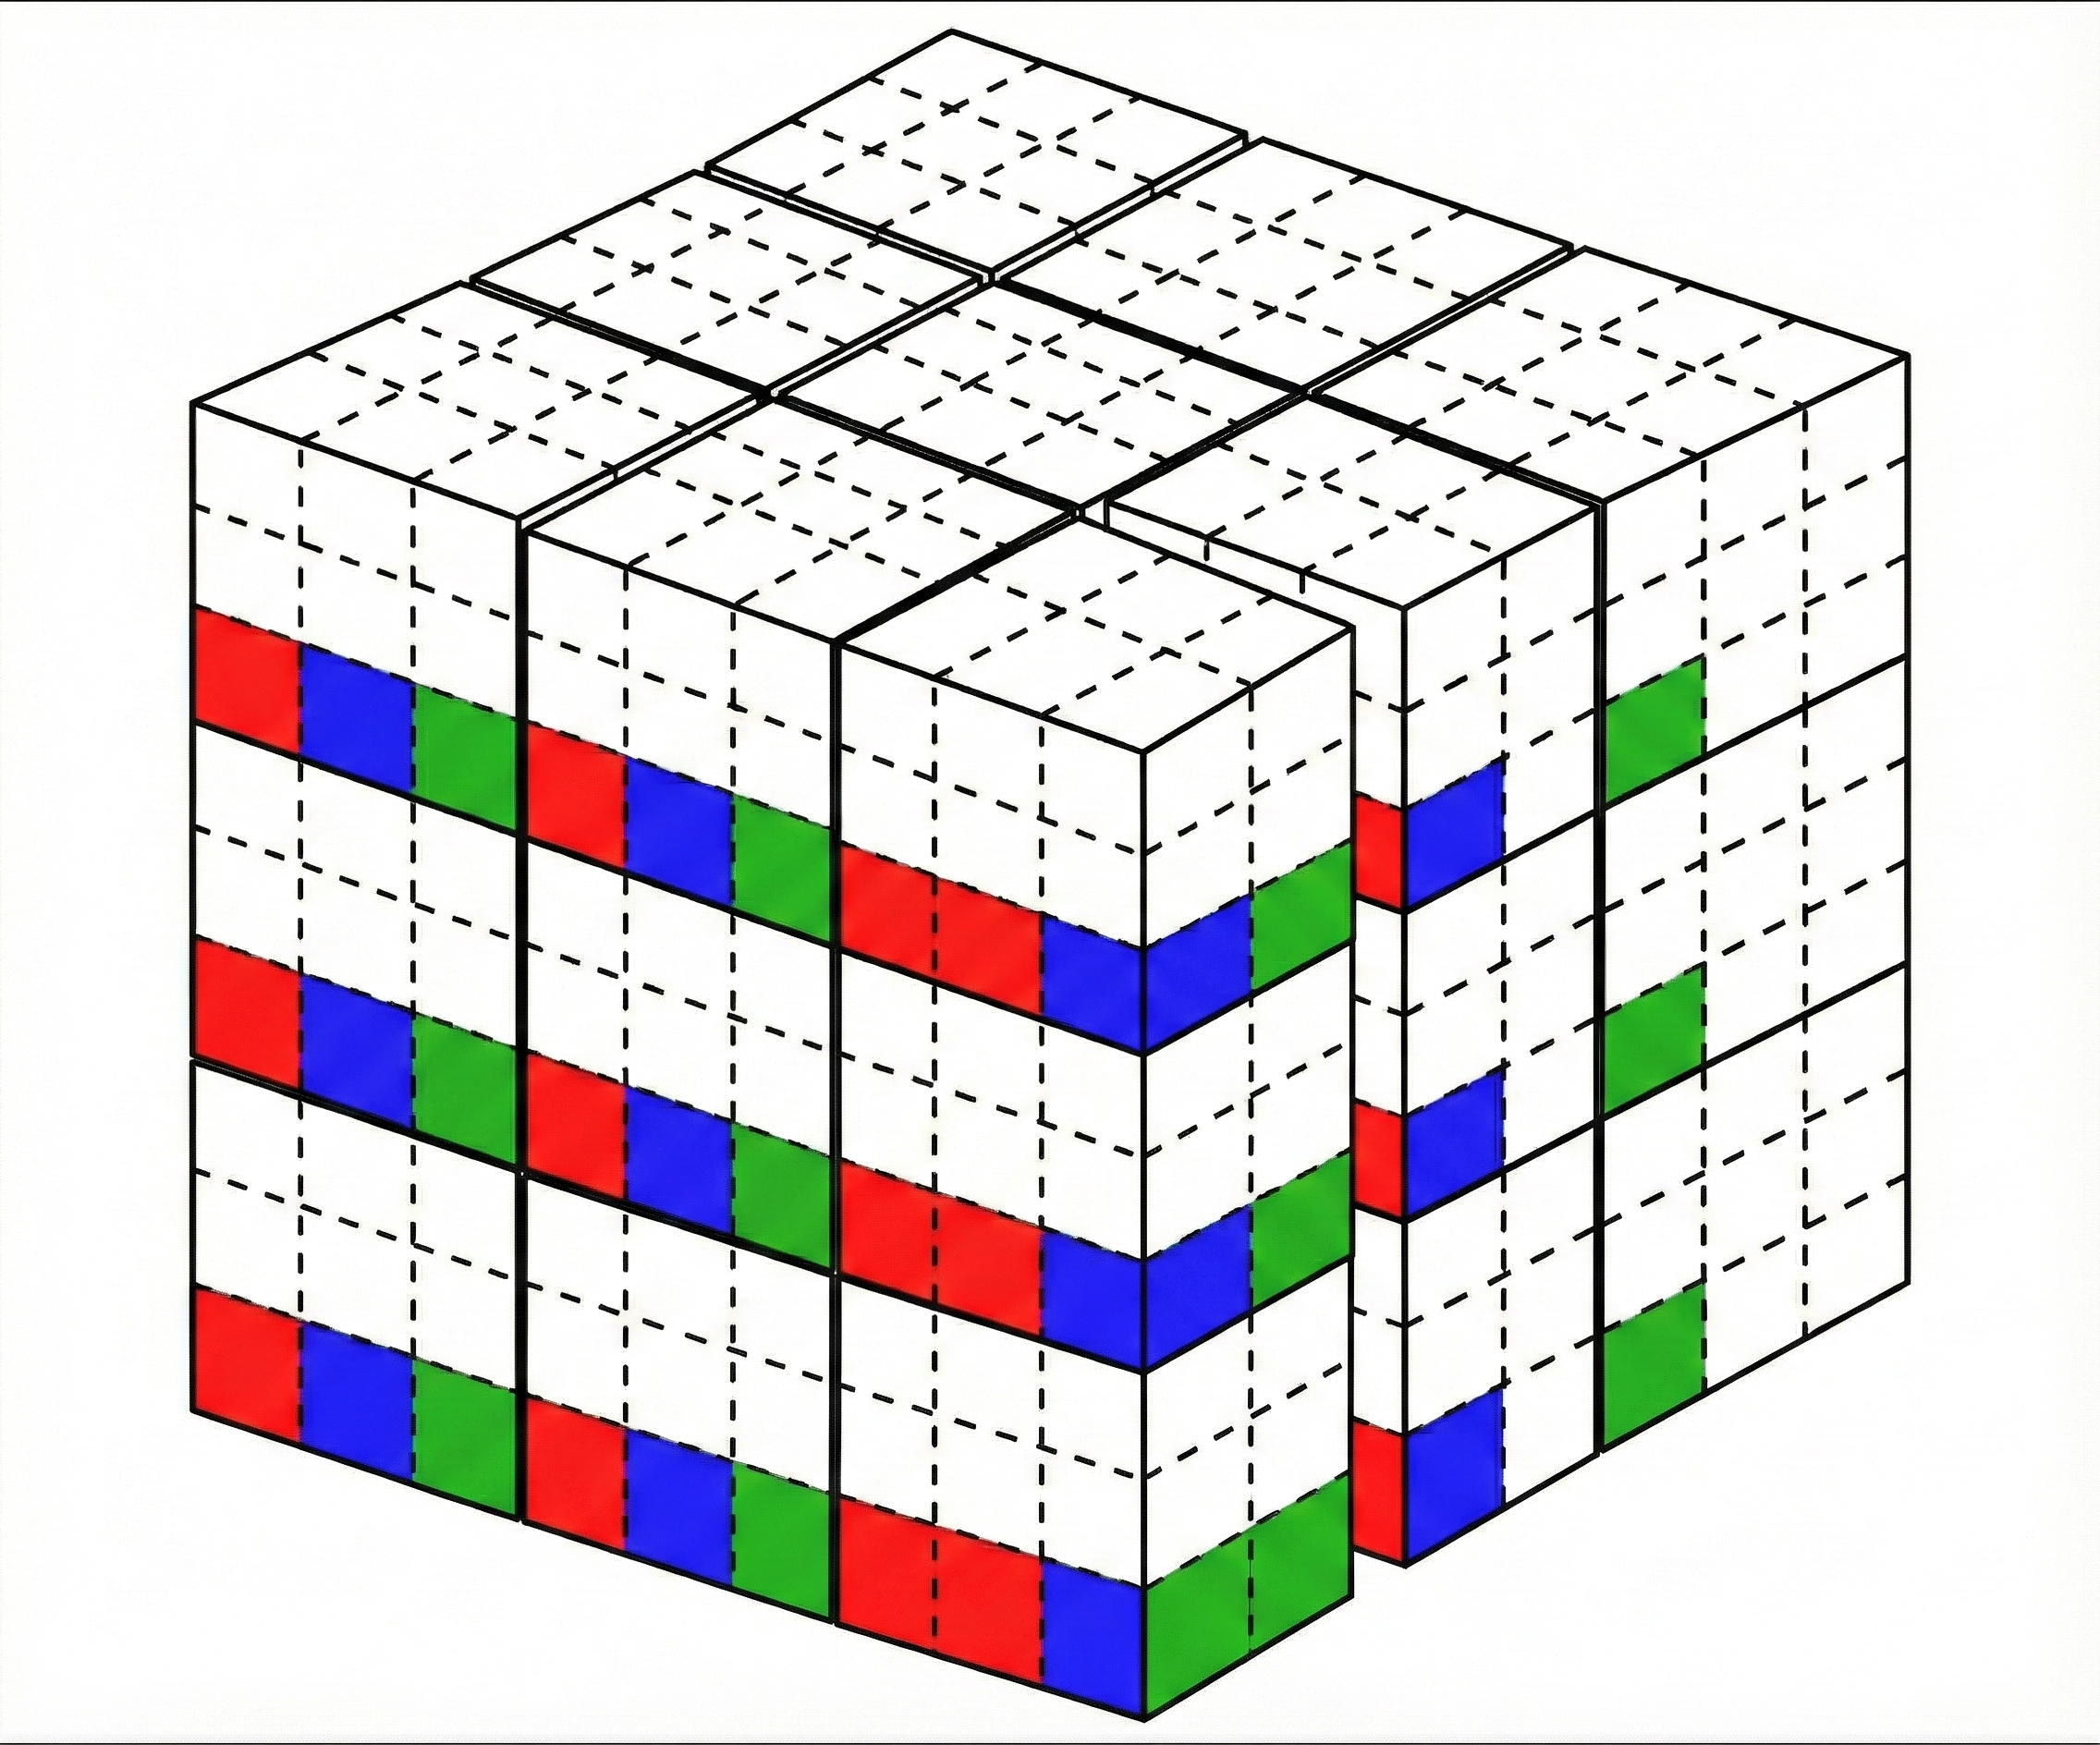
\includegraphics[height=0.35\textheight, keepaspectratio]{img/hyperCube.png}
	\end{frame}
	
\end{document}